
\documentclass[12pt,english]{article}
\usepackage{mathptmx}
\renewcommand{\familydefault}{\rmdefault}
\usepackage[T1]{fontenc}
%\usepackage[utf8]{luainputenc}
\usepackage[letterpaper]{geometry}
\geometry{verbose,tmargin=3cm,bmargin=2cm,lmargin=25mm,rmargin=25mm}
\usepackage{color}
\usepackage{babel}
\usepackage{footnote}
\addto\shorthandsspanish{\spanishdeactivate{~<>}}

\usepackage{array}
\usepackage{longtable}
\usepackage{rotating}
\usepackage{float}
\usepackage{rotfloat}
\usepackage{multirow}
\usepackage{amssymb}
\usepackage{graphicx}
\usepackage{setspace}
\usepackage{nomencl}


%Packages of mindmap

\usepackage[utf8]{inputenc}
%\usepackage{dtklogos}
\usepackage{tikz}
\usetikzlibrary{mindmap,shadows}
% Information boxes
\newcommand*{\info}[4][16.3]{%
  \node [ annotation, #3, scale=0.65, text width = #1em,
          inner sep = 2mm ] at (#2) {%
  \list{$\bullet$}{\topsep=0pt\itemsep=0pt\parsep=0pt
    \parskip=0pt\labelwidth=8pt\leftmargin=8pt
    \itemindent=0pt\labelsep=2pt}%
    #4
  \endlist
  };
}

% Tikz

\definecolor{myblue}{HTML}{020364}
\usetikzlibrary{shapes,arrows,matrix,decorations.pathreplacing,shapes.geometric,positioning}  
% Gantt
\usepackage{pgfgantt}
\usepackage{adjustbox} %Ajustar a la página

% the following is useful when we have the old nomencl.sty package
\providecommand{\printnomenclature}{\printglossary}
\providecommand{\makenomenclature}{\makeglossary}
\makenomenclature
\onehalfspacing
\usepackage{hyperref}
\hypersetup{
    colorlinks = true,
    allcolors = blue,    
}
\makeatletter

%%%%%%%%%%%%%%%%%%%%%%%%%%%%%% LyX specific LaTeX commands.
\DeclareRobustCommand*{\lyxarrow}{%
\@ifstar
{\leavevmode\,$\triangleleft$\,\allowbreak}
{\leavevmode\,$\triangleright$\,\allowbreak}}
%% Because html converters don't know tabularnewline
\providecommand{\tabularnewline}{\\}

%%%%%%%%%%%%%%%%%%%%%%%%%%%%%% Textclass specific LaTeX commands.
\newenvironment{lyxlist}[1]
{\begin{list}{}
{\settowidth{\labelwidth}{#1}
 \setlength{\leftmargin}{\labelwidth}
 \addtolength{\leftmargin}{\labelsep}
 \renewcommand{\makelabel}[1]{##1\hfil}}}
{\end{list}}

%%%%%%%%%%%%%%%%%%%%%%%%%%%%%% User specified LaTeX commands.
\usepackage{lscape}
\addto\captionsspanish{
\def\tablename{Tabla}
\def\listtablename{\'Indice de tablas}
}

\makeatother

\begin{document}

\title{PASSIVE DYNAMIC SYSTEM FOR ENERGY RETURNING ON TRANSTIBIAL PROSTHESIS}
\maketitle

\begin{center}
RESEARCH PROPOSAL 
\par\end{center}

\begin{description}
\item [{NAME:}] \author{Edwin Nikolay Prieto Parrado} \textbf{ID:}C.C 1071162895.
\item [{DEGREE:}] B.E. in Mechatronics - Universidad de San Buenaventura \\ M.Sc. in Mechatronical Engineering - Universidad Militar Nueva Granada.
\item[{POSITION: }] PhD Student of Mechanics and Mechatronics School at Universidad Nacional de Colombia (UNAL) \\ Student Auxiliary Professor at UNAL.
\item[{DATE OF BIRTH: }] February 17th 1987.
\item[{NATIONALITY: }] Colombian
\item[{HOME ADDRESS: }] Calle 12 No. 3 - 05 - La Calera, Cundinamarca, Colombia.
\item[{WORK ADDRESS: }] Carrera 45 No. 26 - 85 - Edificio Uriel Gutiérrez
Bogotá D.C.,  Colombia.
\item[{PHONE NUMBER: }] +57 (1) 3003501177 - +57 (1) 8600428.
\item[{E-mail: }] \href{mailto:enprietop@unal.edu.co}{  enprietop@unal.edu.co}
%\item[{TITLE: }]\emph{{\large PASSIVE DYNAMIC SYSTEM FOR ENERGY RETURNING ON TRANSTIBIAL prosthesis}}


\item [{SUPERVISOR:}] Prof. Dr-Ing. Carlos Julio Cortés Rodríguez.
\item [{CO-SUPERVISOR:}]  Prof. Andrés Tovar PhD.

\textbf{FIELD OF STUDY: } Mechanical Engineering.

 \textbf{SPECIFIC FIELDS OF STUDY:} Computational Modeling, Multibody Rigid and Flexible Dynamics, Lower Limb Prosthesis, Gait Analysis, Biomechanics, Cellular solids.

\textbf{KEYWORDS:} Passive Actuators, Cellular solids, Prosthesis, Ankle joint biomechanics.


\end{description}
\newpage
\renewcommand*\contentsname{Summary}
\tableofcontents
\newpage
%\addcontentsline{toc}{abstract}
\begin{abstract}
Nowadays, Lower Limb Prosthesis (LLP) are changing at a very fast pace, due to technological developments implemented in such devices. In addition, users have new demands about their prosthesis and they require absolute comfort and good performance. Unfortunately, the demand of LLP has risen mostly in third world countries because of the increment of vascular diseases (e.g., Diabetes Mellitus). However, people do not have the enough funds to acquire advanced prosthesis that return the capabilities of walking or jogging in a proper way.

Despite the fact that active prosthesis help people to reduce metabolic cost, those are heavier and more expensive than\emph{ Energy Storage and Return}(ESR\nomenclature{ESR}{Energy Storage and Return prosthesis}) prosthesis devices, produce uncomfortable noises and require more maintenance than passive ones. Moreover, components of the bionic prosthesis (i.e., actuators, battery, gearbox, among others) make the system highly inefficient. As a consequence, a higher quantity of external energy is required to allow the user having enough autonomy for a daily use.

The current work is a Ph.D. thesis, which purpose is manufacturing a novel customizable configuration of transtibial prosthesis. This device will provide the positive work needed for an amputee at the final stance phase through a passive dynamic system, it will take advantage of cellular solids properties for recycling the energetic lost at the initial contact of the gait.

%If the new configuration is successful, the prosthesis will not require the use of an actuator, hence its price and maintenance could be slower than the actives ones and the prosthesis will provide the enough amount of energy for a transtibial amputee at the final stance phase.
\end{abstract}

\printnomenclature{}

\section{MOTIVATION}

The demand of Lower Limb Prosthesis (LLP) is higher every day around the world, due to the constant increment of the principal causes of amputations. According to Ziegler \emph{et al.} \cite{Ziegler-Graham2008}, in the United States of America, amputations in 2008 were caused by vascular diseases (including diabetes) with 53,95\%, followed by trauma (e.g. accidents, warfare, among others) with 44,90\%, and cancer with 1,15\%. They estimated that in 2050 the number of amputees will have risen to 3,6 million \cite{Ziegler-Graham2008}. 

In 2015, the \emph{International Diabetes Federation (IDF\nomenclature{IDF}{International Diabetes Federation})} published the IDF atlas, which announced that the number of people with diabetes is between 340-536 million \cite{IDF2015}. Moreover, they estimated that this sickness will have affected 642 million of people worldwide by 2050.
  
It is believed that diabetes affects mostly the lower limbs, producing potential risks of suffering peripheral arterial illness, diabetic foot and, as a result, an amputation. The possibility of suffering an amputation will depend on race, gender, and age of the population, being different in many countries. Below, Fig. \ref{fig:N=0000FAmero-de-amputaciones} shows the number of amputations per 100.000 habitants caused by diabetes.
\begin{figure}[H]
\begin{centering}
\includegraphics[scale=0.5]{ampperyear}
\par\end{centering}

\caption{\label{fig:N=0000FAmero-de-amputaciones}Population affected per 100.000 inhabitants during a specific period of time in each country. Adapted from Kroger and Knut \cite{KrogerKnut2015}.}

\end{figure}


Despite the lack of statistics of amputations in all countries, diabetes is considered the main cause of amputation around the world.

Even though bionic prosthesis supply more amount of energy than \emph{ Energy Storage and Return}(ESR) at final stance phase, those are extremely expensive for developing countries. Thus, we have to take into account those communities with a limited economic capacity to get those devices. In consequence, third world countries sacrifice good Quality of Life (QoL\nomenclature{QoL}{Quality of Life}) with low technology prosthesis \cite{Lemoyne}.

To sum up, contributing to the development of prosthetic devices for lower limbs has great relevance for improving disorders in pathological gait and therefore obtain better QoL. The strategy to recover the absence of limbs work is recycling energy of Initial Contact (IC\nomenclature{IC}{Initial Contact}) and return it during final stance phase. It is thought that this strategy could be cheaper than prosthesis with active actuators inside. 




\section{\label{sub:Estado-del-conocimiento:}STATE OF THE ART}


\subsection{State of the Art about Ankle-Foot Prosthesis}

This motivation encourages research on devices that restore energy loss in gait as efficiently as possible. Moreover, replacing ankle joint is a complex task because it should be able to manage its stiffness regardless the terrain or the type of gait. Great technological advances in prosthesis have been made worldwide. There are clearly two kinds of strategies in foot prosthesis: ESR prosthesis, which state-of-the-art was described by Versluys \emph{et al.} \cite{Versluys2009}; and bionic prosthesis, described by Cherelle \emph{et al.} \cite{Cherelle2014a} on what is considered a bionic prosthesis and, consequently, their types. Fig. \ref{fig:Categorizaci=0000F3n-seg=0000FAn-Cherelle} depicts a generalized representation of foot prosthesis classes, where the most implemented foot prosthesis  is the SACH, despite not having returning energy benefits in gait.

\begin{figure}[H]
\begin{centering}
\includegraphics[scale=0.68]{GeneracionesprotesisEng}
\par\end{centering}

\caption{\label{fig:Categorizaci=0000F3n-seg=0000FAn-Cherelle} Generalized categorization of ankle-foot prosthesis according to Cherelle \emph{et al.}\cite{Cherelle2014a} and Versluys \emph{et al.} \cite{Versluys2009}. From left to right: SACH foot, sagital degree of freedom foot, OSSUR$\circledR$ flex foot, Echelon foot$\circledR$, Proprio foot from OSSUR$\circledR$ and BiOM$\circledR$ from iWalk Inc.}
\end{figure}

Principal strengths and weaknesses in prosthesis to date have been found, both for ESR and bionic prosthesis, which are depicted in Tables \ref{tab:Fortalezas,-debilidades-ESR}, and \ref{tab:Fortalezas-de-las-activas} - \ref{tab:Debilidades-pr=0000F3tesis-activas}, respectively. 

Furthermore, weaknesses in prosthesis generate biomechanical disorders in gait, which are mentioned in Table \ref{tab:Alteraciones-biomec=0000E1nicas-ESR} for ESR and Table \ref{tab:Alteraciones-biomec=0000E1nicas-activas} for bionics.

\begin{center}
\begin{table}[H]
\caption{\label{tab:Fortalezas,-debilidades-ESR}Strengths and weaknesses on ESR prosthesis}


\centering{}%
\begin{tabular}{|>{\raggedright}p{3cm}|>{\centering}p{13cm}|}
\hline 
\multirow{2}{3cm}{\textbf{Passive prosthesis strengths}} & The price of ESR is cheaper than bionic ones.\tabularnewline
\cline{2-2} 
 & Good source of positive external work at final stance phase without requiring batteries \cite{Zelik2014}.\tabularnewline
\hline 
\hline 
\multirow{5}{3cm}{\textbf{Passive prosthesis weaknesses}} & It can only react at final compression of material while actives act and react. \cite{Varol2010}.\tabularnewline
\cline{2-2} 
 & Significant ankle power difference between the affected and unaffected sides during ankle-powered plantar flexion. \cite{Au2009,herr2014powered}.\tabularnewline
\cline{2-2} 
 & Poorer shock absorption on affected side \cite{Au2008}. \tabularnewline
\cline{2-2} 
 & It cannot replicate the positive work phases of the human joint. \cite{Martinez-Villalpando2009,Esposito2015}.\tabularnewline
\cline{2-2} 
 & As prosthetic foot deforms during loading, it will exert a braking effect on the \emph{Center of Mass} (CoM\nomenclature{CoM}{Center of Mass}) progression. \cite{DeAsha2014}.\tabularnewline
\hline 
\end{tabular}
\end{table}

\par\end{center}

\begin{center}
\begin{table}[H]
\caption{\label{tab:Alteraciones-biomec=0000E1nicas-ESR}Biomechanical disorders in ESR prosthesis users}


\centering{}%
\begin{tabular}{|l|>{\centering}p{15cm}|}
\hline 
\multirow{8}{*}[-17mm]{\begin{turn}{90}
\textbf{Biomechanical disorders.}
\end{turn}} & Users expend between 20\% and 30\% more metabolic power to walk.
\cite{Au2009,Schmalz2002}.\tabularnewline
\cline{2-2} 
 & Users walk between 30\% and 40\% slower the same distance in comparison with an able-bodied person. \cite{Au2009,Buckley1997,Herr2010,Gates2013,Hill2013a,Schmalz2002}.\tabularnewline
\cline{2-2} 
 & Users show asymmetric patterns in gait \cite{Au2009,Martinez-Villalpando2011,Hill2013a}.\tabularnewline
\cline{2-2} 
 &  Hip extension, knee flexion and ankle dorsi-flexion on the unaffected side are higher than normal \cite{Morgenroth2011, Bateni2002}. \tabularnewline
\cline{2-2}
& Affected limb has higher stance phase time, higher step length, less swing phase time and less inertia moment than unaffected side.\cite{Mattes2000}.\tabularnewline
\cline{2-2} 
 & People with unilateral transtibial amputation have an increased susceptibility to knee osteoarthritis. \cite{Grabowski2013}.\tabularnewline
\cline{2-2} 
& Biomechanical disorders in gait might be the main cause of dorsal-lumbar pain \cite{Devan2014}. \tabularnewline
\hline 
\end{tabular}
\end{table}

\par\end{center}

In spite of the fact that bionic prosthesis provide more benefits than passive ones in terms of dynamic improvements in gait, nowadays those prosthesis present disadvantages and some dynamic disorders in gait (See Table \ref{tab:Alteraciones-biomec=0000E1nicas-activas}).  

\begin{center}
\begin{table}[H]
\caption{\label{tab:Fortalezas-de-las-activas}Bionic prosthesis strengths in comparison to passive ones}


\begin{tabular}{|c|>{\centering}p{15cm}|}
\hline 
\multirow{8}{*}[-6mm]{\begin{turn}{90}
\textbf{Bionic prosthesis strengths}
\end{turn}} & The system replaces musculoskeletal work in gait \cite{Varol2010}. \tabularnewline
\cline{2-2} 
 & It is capable of recognizing different types of terrain and velocities of gait \cite{Lawson2011}. \tabularnewline
\cline{2-2} 
 & It is capable of producing positive mechanical power \cite{Martinez-Villalpando2009}.\tabularnewline
\cline{2-2} 
 & It reduces the metabolic demand up to 16\% \cite{Herr2010,Esposito2015}.\tabularnewline
\cline{2-2} 
 & Present more stable trajectory in comparison to passives \cite{Hill2013a}.\tabularnewline
\cline{2-2} 
 & Subjects had a 10\% faster self-selected walking speed on uneven ground when wearing the powered compared with ESR. \cite{Gates2013}.\tabularnewline
\cline{2-2} 
 & Reductions in peak impact resultant force, impact resultant force loading rate, peak heel-strike foot pressure and peak knee external adduction moment when comparing powered ankle-foot prosthesis to the conventional passive prosthesis. \cite{Hill2013a}.\tabularnewline
\cline{2-2} 
 & Decreasing in peak resultant force and adductor knee moments on unaffected limb \cite{Grabowski2013}.\tabularnewline
\hline 
\end{tabular}
\end{table}

\par\end{center}

\begin{center}
\begin{table}[H]
%\begin{savenotes}


\caption{\label{tab:Debilidades-pr=0000F3tesis-activas} Recent weaknesses on powered prosthesis}


\begin{tabular}{|l|>{\centering}p{15cm}|}
\hline 
\multirow{9}{*}[-10mm]{\begin{turn}{90}
\textbf{Powered prosthesis weaknesses}
\end{turn}} & \centering{} Electric-based machines make noises. \cite{boston}.\tabularnewline
\cline{2-2} 
 & \centering{} Most of them are not scalable, pediatric users cannot use it. \cite{BIOMASME}.\tabularnewline
\cline{2-2} 
 & It still requires biomimetic ankle intervention. \cite{Hill2013a}.\tabularnewline
\cline{2-2} 
 & High cost, up to U\$40.000 - U\$50.000. Price of BiOM® according to Boston Magazine\cite{boston} could be around U\$ 40.000. The Proprio® prosthesis from Ossur could be around U\$25.000 \cite{bloomberg}. On the other hand, an ESR prosthesis is between U\$ 500 and U\$3.000.\tabularnewline
\cline{2-2} 
 & Most of ESR prosthesis are lighter than powered.\tabularnewline
\cline{2-2} 
 & It requires more maintenance than passive ones.\tabularnewline
\cline{2-2} 
 & Technical parameters need tuning (i.e. power, torque, cycle times, etc) according to anthropometric requirements. \tabularnewline
\cline{2-2} 
 & System is inefficient since mechanical design incurs in energetic losses \cite{boston, Cherelle2014a}, thus autonomy is lower than in passive prosthesis.\tabularnewline
\cline{2-2} 
 & Specific implementation of control strategies - as Reis mentioned in \cite{Reis2016} - are needed for powered prosthesis. Consequently, hardware and software are more demanding. \tabularnewline
\hline 
\end{tabular}
%\end{savenotes}

\end{table}

\par\end{center}

\begin{center}
\begin{table}
\caption{\label{tab:Alteraciones-biomec=0000E1nicas-activas}Recent biomechanical disorders on powered prosthesis}


\centering{}%
\begin{tabular}[b]{|>{\raggedright}p{3cm}|>{\centering}p{125mm}|}
\hline 
\multirow{2}{3cm}{\textbf{Biomechanical disorders}} & Since the user gait is more dynamic, the pressure in stump is higher than in ESR users. Hence, the risk of suffering ulcers, dermatitis or any trauma in that area, is higher. \cite{Wolf2009}\tabularnewline
\cline{2-2} 
 & To date, it only has been designed for adult population. It is not suitable for children \cite{BIOMASME}.\tabularnewline
\hline 
\end{tabular}
\end{table}

\par\end{center}

ESR prosthesis are not able to reestablish the dynamic walking nor the metabolic cost, due to the absence of the lower limb. On the other hand, powered prosthesis have restored the positive work needed to return the controlled energy and satisfy the quasi-stiffness slope \cite{hansen2014ankle, Eshraghi2013} of lost ankle. However, methods to reestablish the energy are highly inefficient \cite{Cherelle2014a}, making those devices more complex and expensive compared to ESR.  

Literature has reported a variety of actuators, which are divided in: stiff actuators and Compliance actuators. The pros and cons are described in \nameref{sec:Ap=0000E9ndice-B:}. According to Vanderborght \emph{et al.} \cite{Vanderborght2013}, those actuators will undergo continuous development aiming to achieve the best energetic efficiency, stability, autonomy and a regular walking.

Even though some actuators have not been made yet, because of the geometric constraints to implement those components, some others have been implemented in commercial prosthesis (e.g. Series Elastic Actuator). That kind of actuators have shown an improvement in walking. Nevertheless, high electric power is required by the actuator, thus autonomy \footnote{Autonomy is calculated by number of steps until the powered prosthesis discharges. Generally, It must satisfy between 3000 to 5000 steps per day\cite{Grabowski2013}.} is reduced.      

Two variables were taken into account by Grimmer \cite{Grimmer2012, Grimmer2014} and Eslamy\cite{Eslamy2013, Eslamy2014} to determine efficiency on actuators. Those are \emph{Peak Power (\nomenclature{PP}{Peak Power}PP)} and  \emph{Energetic Requirement} (\nomenclature{ER}{Energetic Requirement}ER). The more PP and ER per cycle in the motor, the more electric energy required. 

Some actuators mentioned in Appendix A were studied to verify the requirements of the motor, and identify the more efficient. Fig. \ref{fig:Variables-mec=0000E1nicas-actuadores} shows the results of the most popular actuators used in foot prosthesis for a subject of 75 kg of mass and cadence at 1 m/s.

\begin{figure}[H]
\begin{centering}
\includegraphics[scale=0.55]{20160414035751}
\par\end{centering}

\caption{\label{fig:Variables-mec=0000E1nicas-actuadores}Mechanical requirements of varied prosthetic actuators. Results were obtained by mathematical modeling of each one \cite{Cherelle2014a}. Nomenclature: PEA: Parallel Elastic Actuator, CPEA: Clutched PEA, SEA (Opt. ER): SEA actuator focused on optimizing ER,
SEA (Opt. PP): SEA actuator focused on optimizing PP, EEA: Explosive Elastic Actuator. }
\end{figure}

It must be taken into account that the power required for each actuator does not consider energy losses made by the system, which are around 50-60\%; Hence, 600W are needed to generate pure power of 287 W by the motor \cite{Cherelle2014a}.


Based on the foregoing, from the gait analysis, it has been found that energy dissipation occurs when the velocity vector of the COM is redirected at each step-to-step transition \cite{Donelan2002}. In other words, the stance leg in every gait cycle, acts similarly to an inverted pendulum, in order to support the body COM. Consequently, when transition is made - in double support phase - the COM velocity is redirected and energy is lost at collision of the heel with ground \cite{Collins2010}. A graphic explanation can be seen in Fig. \ref{fig:(A)-Representaci=0000F3n-de}A.

Therefore, Collins and Kuo \cite{Collins2010} built a prosthetic foot which initially recycled the energy lost at initial contact of the gait through the implementation of a compression spring. This spring stores the energy until late stance phase of gait to finally release it, with the purpose of providing positive work to amputees. Nevertheless, neither shock absorption was reduced, nor the system provided all energy needed to restablish a regular gait.

\begin{figure}
\begin{centering}
\includegraphics[scale=0.5]{RecycledEng}
\par\end{centering}

\caption{\label{fig:(A)-Representaci=0000F3n-de}\emph{"(A) The stance leg acts similarly to an inverted pendulum to support the body center of mass. The center of mass velocity is redirected between steps when the other leg contacts the ground with a dissipative collision. (B) The rate of work performed on the center of mass by ideal pendulum-like legs vs. stride time. Work is theoretically minimized by pushing off impulsively (indicated by arrows) just before the opposite leg’s collision (step-to-step transition indicated by darkened intervals above time axis). (C) Conceptual plot of center of mass work rate for human-like legs vs. stride time. Imperfectly rigid legs will smooth out the impulses, but the collision (hatched area) is nevertheless a possible source of energy for recycling if it can be captured, stored, and later released for push-off." }Paragraph and figure taken from Collins and Kuo\cite{Collins2010}.}


\end{figure}

In general, powered prosthesis follow the next procedure: an ESR foot is used as base, later the actuator is implemented for push-off; Then, a control strategy is needed for its use and finally a battery is installed as source of power. Based on the previous technique for restoring limb loss, a question arised: what other strategy could be implemented in prosthesis so that, it obtains a better efficiency?.  

To sum up, pathologies caused by lower limb amputations befall in extra expenditure of energy (i.e. metabolic cost) for patients, due to the absence of \emph{triceps surae} group, which generates approximately 80\% of the work needed for push-off. In spite of the fact that ESR prosthesis provide positive work at final stance phase, to date those are not able to provide all the needed work. On the other hand, powered prosthesis are capable of supplying positive work needed by an amputee, but, that type of prosthesis has lower autonomy than ESR since the integrated actuator is inefficient. Hence, the necessity of the design of passive dynamic systems (concept defined by McGeer \cite{mcgeer1990passive}) for foot prosthesis emerged. 

\subsection{Additive Manufacturing on Prosthesis}

The evolution of technological development in medicine is growing faster nowadays, from manufacturing prototypes for academic purposes to cloning a cell, a tissue or an organ to implant \cite{Michalski2014}. All the above range of facilities are due to Additive Manufacturing \nomenclature{AM}{Additive Manufacturing} - well known as 3D printing -, which principle is based on making pieces layer by layer, on the basis of CAD\nomenclature{CAD}{Computer Aided Design} models. AM pros and cons in comparison to traditional manufacturing are well described by Weller \emph{et al.}\cite{Weller2015} and Diegel \emph{et al.} \cite{Diegel2014}.  

Those advantages suited the necessities of prosthesis makers, who demonstrated that mechanical properties of printable materials accomplish the task demanded by a foot prosthesis \cite{South2010, Yap2015}. It is believed that concepts of prosthesis with AM will adapt new shapes and could possibly change its mechanical properties  dynamically, due to the combination of self-assembly technique and 3D printing. Some experiments have been reported by Tibbits \emph{et al.}\cite{Tibbits2014,Raviv2014} and Yu \emph{et al.}\cite{Yu2015}.

Even though few foot prosthesis are made from AM, all of them have uniform mechanical properties all over its structure, This affects negatively the accomplishment of elastic properties needed for satisfying ankle quasi-stiffness on the prosthesis. In addition, given the ability to add material freely in AM without manufacturing penalties, the shape and geometry could be adapted easily in case of changes in the anthropomorphicity of users (i.e. pediatric users).

\subsection{Optimal Design}

The trend of engineers to build \emph{ Finite Element Models}(FEM\nomenclature{FEM}{Finite Element Models})--- to simulate how complex products will perform --- has increased. Moreover, this method allows the designer to modify some changes in order to get better results, encouraging the implementation of optimization techniques in the most critical obstacles over the design \cite{Forrester2008}. 

In the mechanical design, optimization techniques such as topology optimization \cite{Sigmund2001, Andreassen2011}, shape optimization \cite{Munk2015} and topometry optimization are being exponentially used along the last two decades.

Furthermore, meta-analysis algorithms such as \emph{Multi Disciplinary Optimization} (MDO\nomenclature{MDO}{Multi Disciplinary Optimization}), \emph{Multi Objective Optimization Algorithms} (MOOA\nomenclature{MOOA}{Multi Objective Optimization Algorithms}) and \emph{Multi Objective Evolutionary Algorithms} \cite{Wnag2006} (MOEA\nomenclature{MOOA}{Multi Objective Evolutionary Algorithms}) have helped to reach a faster answer in the search for the optimal point in the design \cite{Suresh2010, Huang2010}. 

%\subsection{Muscle-Skeletal computational Models:}

%Part of the biomechanical parameters mentioned in previous sections cannot be easily measured or might not be seen with the naked eye. 



\section{PROBLEM STATEMENT}

\begin{itemize}
\item The recent passive prosthesis for transtibial amputees produce disorders in the dynamic parameters of the gait, owing to the absence of positive work of the limb loss. 
\end{itemize}

\subsection{Research Question}

Which passive ankle-foot prosthesis based on cellular solids configurations, will generate the positive work needed for push-off, taking advantage of the energy lost at initial contact of the gait?

\subsection{Hypothesis}

A passive dynamic system (compound of cellular solids) within a passive ankle-foot prosthesis, configured to store energy in a controlled manner at initial contact of the early stance phase, will enable to return the stored energy after dorsiflexion phase.



\subsection{General and Specific Objectives}

\subsubsection{General Objective} To suggest an ankle-foot prosthesis being able to generate - through a passive dynamic system - the positive work needed for push-off after dual-flexion phase, taking advantage of the energy lost at initial contact of the gait.

\subsubsection{Specific Objectives}
\begin{enumerate}
\item Identify biomechanical parameters and the work-loop slope of ESR prosthesis users and non-amputees aiming to obtain the ankle quasi-stiffness of both cases.

\item Obtain a preliminary model of the ankle-foot prosthesis capable of storing energy (during initial contact until late dual-flexion phase), and returning it at dorsi-flexion phase in a controlled manner through the passive dynamic system.

\item Determine detailed configurations of cellular solids that accomplish the requirements of the preliminary model.
\item Validate the dynamic model of the ankle-foot prosthesis in comparison to an ESR prosthesis. \end{enumerate}

\subsection{Methodology and Activities}

The methodological procedure will be carried out through the extraction of statistical data, in order to obtain the ankle quasi-stiffness slope of prosthesis users and non-amputees, so as to compare the energetic gap between those cases. On the other hand, an \emph{in-silico} process to design the prosthesis is needed to propose the concept and verify its functionality. This simulation process will be done with the tentative computational framework proposed in Figure \ref{Marco-computacional}. 

\begin{figure}[ht]
\begin{centering}
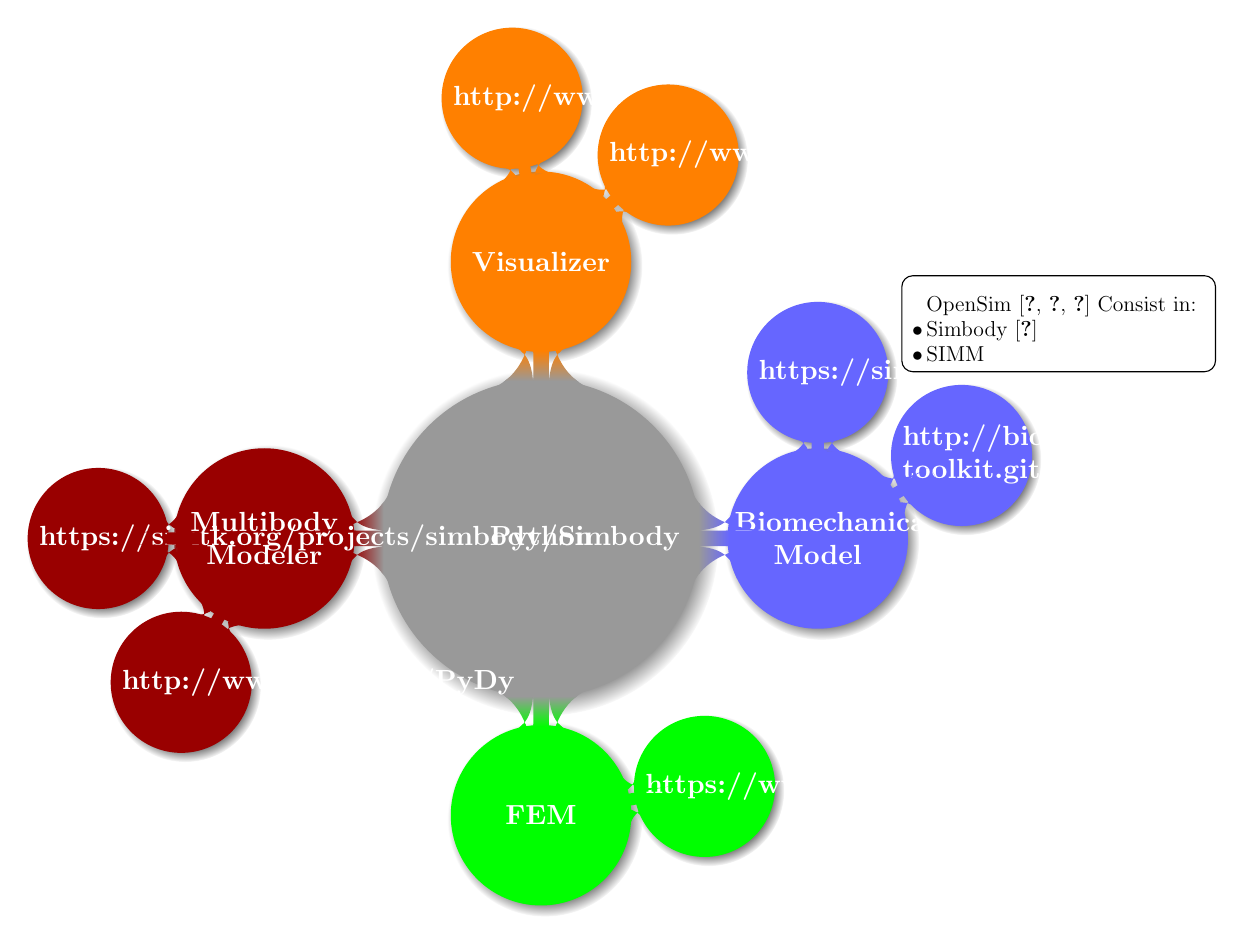
\begin{tikzpicture}[ every annotation/.style = {draw,
                     fill = white, font = \large,text width=4em}]
  \path[mindmap,concept color=black!40,text=white,
    every node/.style={concept,circular drop shadow},
    root/.style    = {concept color=black!40,
      font=\normalsize\bfseries,text width=6em},
    level 1 concept/.append style={font=\normalsize\bfseries,
      sibling angle=90,text width=6em,
    level distance=10em,inner sep=0pt},
    level 2 concept/.append style={font=\bfseries,level distance=6em},
  ]
  node[root] {Python} [clockwise from=0]
    child[concept color=blue!60] {
      node {{Biomechanical Model}} [clockwise from=90]
        child { node (goForum) {\href{https://simtk.org/projects/opensim}{OpenSim}} }
        child { node (goWiki) {\href{http://biomechanical-toolkit.github.io/}{BTK}} }
    }
    child[concept color=green!120] {
      node[concept] {{FEM}}
        [clockwise from=10]
      child { node[concept] {\href{https://www.csc.fi/web/elmer}{ELMER}} }
    }
    child[concept color=red!60!black] {
      node[concept] {{Multibody Modeler}}
        [counterclockwise from=180]
      child { node[concept] {\href{https://simtk.org/projects/simbody/}{Simbody}}}
      child { node[concept] {\href{http://www.pydy.org/}{PyDy}} }
      }
    child[concept color=orange] {
      node[concept] {{Visualizer}}
        [clockwise from=100]
        child { node[concept] {\href{http://www.vtk.org/documentation/}{VTK}}
        }
        child { node[concept] {\href{http://www.paraview.org/overview/}{Paraview}}
        }};
    \info{goForum.north east}{above,anchor=west,xshift=1em}{%
      \item[] OpenSim \cite{Delp2007,Reinbolt2011,Seth2011} Consist in:
      \item Simbody \cite{Sherman2011}
      \item SIMM
    }


\end{tikzpicture}
\caption{\label{Marco-computacional} A computational framework of the proposed methodology. Click on the hyperlinks to see more details of every open-source software.}
\end{centering}
\end{figure}
\begin{figure}[ht]
\begin{centering}
\includegraphics[scale=0.4]{HicksMethod}
\par\end{centering}

\caption{\label{fig:Proceso-validaci=0000F3n-y}Best validation and verification practices for biomechanical models. Taken from Hicks \emph{et al.} \cite{Hicks2014}}
\end{figure}
\begin{description}
\item [{Objective}]  \textbf{1:} Identify biomechanical parameters and the work-loop slope of ESR prosthesis users and non-amputees aiming to obtain the ankle quasi-stiffness of both cases.
\item [{Methodology:}] Obtaining the most important biomechanical parameters (as mentioned by Sagawa \cite{Sagawa2011}) for ankle quasi-stiffness slope  through extraction of data in order to compare the energetic demand of an ESR user with a non-amputee.
\end{description}

\begin{description}
%\vspace{10 mm}
\item [{Activities:}]~\end{description}
\begin{enumerate}
\item To search in literature the most useful data and filter it.
\item To obtain biomechanical parameters for getting different ankle quasi-stiffness slopes of different ESR and able-bodied patients. 
\item To make the biomechanical model of each subject with the purpose of acquiring non-measurable variables and predicting biomechanical behavior through forward dynamic technique in specific software like OpenSim$\circledR$.
\item To obtain ankle quasi-stiffness slope by the combination of kinetic and kinematic variables.
\item To obtain energetic loss in the collision at initial contact of the gait.
\item To verify biomechanical models with similar publications in literature. \end{enumerate}
\begin{description}
\item [{Objective}]  \textbf{ 2: } Obtain a preliminary model of the ankle-foot prosthesis capable of storing energy (during initial contact until late dual-flexion phase), and returning it at dorsi-flexion phase in a controlled manner through the passive dynamic system.
\item [{Methodology:}] To suggest the preliminary model of the ankle-foot prosthesis capable of storing energy, The design of that model will be iterated through FEM tools combined with flexible multi-body simulations until reaching the optimized configuration of sub-domains conditioned to the anthropometric volume. 

\end{description}

\begin{description}
\item [{Activities:}]~\end{description}
\begin{enumerate}
\item To divide the biomechanical models into gait sub-phases to analyze each one separately.
\item To determine the geometry restricted to the anthropometric volume with CAD software (e.g. Inventor$\circledR$).
\item To define the elastic configuration needed to store the energy at each sub-phase of gait.
\item To split the global domain into different sub-domains and define constitutive equation of each sub-domain according to the required energetic storage specifications. (PyDy$\circledR$/Simbody$\circledR$ y ELMER$\circledR$).
\item To design the mechanism, which stores energy from initial contact to mid-stance phase with the aim of returning it at late stance phase. 
\item To verify flexible multi-body models with FEM tools.\end{enumerate}

\begin{description}
\item [{Objective}]  \textbf{ 3: }To determine detailed configurations of cellular solids that accomplish the requirements of the preliminary model.
\item [{Methodology:}] Departing from the obtained configuration, a cellular material might be applied to each sub-domain to equalize the mechanical requirements of the model obtained in the previous objective.
\item [{Activities:}]~\end{description}
\begin{enumerate}
\item To obtain a cellular solid configuration to accomplish the specific elastic properties of each sub-domain.
\item To verify the mechanical behaviour of each sub-domain with its cellular solid configuration.  
\item To verify the structural resistance of the entire model submitted to static loads through FEM or DES\nomenclature{DES}{Discrete Element Method} tools.
o FEM.
\item To get the ankle quasi-stiffness slope of the new configuration with the forward dynamics technique in the biomechanical model mentioned above.
\end{enumerate}
\begin{description}
\item [{Objective}]  \textbf{ 4:} Validate the dynamic model of the ankle-foot prosthesis in comparison to an ESR prosthesis.
\item [{Methodology:}] Manufacturing the ankle-foot prosthesis through 3D printing techniques in order to validate the storage and return efficiency. Finally, we will compare with an ESR prosthesis user.
\item [{Activities:}]~\end{description}
\begin{enumerate}
\item Accomplish the medical ethic procedure and request permission for the validation process.
\item Select ESR prosthesis users and adapt them to the new prototype.
\item To collect biomechanical parameters of ESR users as well as of the new prototype. 
\item To compare the delivered work during the step-to-step transition in gait with the new concept, the standard ESR prosthesis, and able-bodied patients.
\item To determine the energy storage through the strain measurement of each sub-domains by optic equipment like \href{http://www.gom.com/industries/medical-technology/biomechanics.html}{GOM}.
\item To evaluate significant biomechanical differences between the new concept of prosthesis and ESR prosthesis on all over the gait.
\item To conclude results and evaluate future work. 
\end{enumerate}

\subsection{Implications and Expected Results}

The level of impact in this research consist in a new concept of transtibial prosthesis capable of storing energy in many instances of the gait to return it in a controlled manner at final stance phase without the need of external power sources, stepping up energetic contribution in comparison with an ESR prosthesis.

On the other hand, ankle quasi-stiffness depends directly on weight and step length, therefore a customized ankle-foot prosthesis is needed to solve metabolic cost problems in users. In addition, uniform mechanical properties of ESR prosthesis are not able to reproduce the ankle quasi-stiffness properly. The more deficient ankle quasi-stiffness, the more metabolic cost is demanded. In contrast, powered prosthesis generate the positive work needed for an amputee, but its efficiency is much lower than ESR and, as a result, autonomy is reduced. Despite the fact that its electronic components help to get the prosthesis controlled, it increases the cost and third-world countries, where the most amount of amputees live, are not able to acquire one of these.

Moreover, new manufacturing techniques are able to customize the prosthesis according to the anthropometry of users and their specific biomechanical disorders; Hence, we can reach specific elastic properties at different sub-domains through a cellular solid configuration, which have never been seen in any kind of prosthesis.

\newpage
\section{SCHEDULE }

\begin{ganttchart}[
x unit=0.3cm,
y unit title=0.7cm,
y unit chart=0.8cm,
vgrid,
time slot format=isodate-yearmonth,
compress calendar,
title/.append style={draw=none, fill=myblue},
title label font=\footnotesize\sffamily\bfseries\color{white},
title label node/.append style={below=-1.6ex},
title left shift=.05,
title right shift=-.05,
title height=1,
bar/.append style={draw=none, fill=green!75},
bar height=.6,
bar label font=\normalsize\color{black!50},
group right shift=0,
group top shift=.6,
group height=.3,
group peaks height=.2,
bar incomplete/.append style={fill=brown}
]{2016-04}{2018-12}
\gantttitlecalendar{year} \\
\ganttbar[
progress=100,
bar progress label font=\small\color{black},
bar progress label node/.append style={right=4pt},
bar label font=\footnotesize\color{black!50},
name=pp
]{Doctoral Proposal}{2016-04}{2016-06} \\
\ganttset{progress label text={}, link/.style={black, -to}}
\ganttgroup{Objective 1}{2016-06}{2017-03}\\ 
\ganttbar[progress=100, name=T1A]{Obtaining data from the literature}{2016-06}{2016-07} \\
\ganttbar[progress=100, name=T1A]{Filtering data}{2016-07}{2016-08} \\
\ganttbar[progress=100, name=T1A]{Obtaining biomechanical model}{2016-08}{2016-10} \\
\ganttbar[progress=100, name=T1A]{Getting ankle quasi-stiffness}{2016-10}{2016-12} \\
\ganttbar[progress=100, name=T1A]{Verificating results}{2017-01}{2017-03} \\
\ganttgroup{Objective 2}{2017-06}{2017-12} \\
\ganttbar[progress=0, name=T2A]{Including loads and constrains}{2017-06}{2017-08} \\
\ganttbar[progress=0, name=T2A]{Determining geometries}{2017-08}{2017-10} \\
\ganttbar[progress=0, name=T2A]{Optimizing sub-domains}{2017-10}{2017-07} \\
\ganttbar[progress=0, name=T2A]{Obtaining preliminary design}{2017-07}{2017-10} \\
\ganttbar[progress=0, name=T2A]{Simulate preliminary design}{2017-08}{2017-12} \\
\ganttgroup{Objective 3}{2017-10}{2018-06} \\
\ganttbar[progress=0]{Cellular solids configurations}{2017-10}{2018-01}\\
\ganttbar[progress=0, name=T2A]{Verifying energetic storage}{2017-12}{2018-04} \\
\ganttbar[progress=0, name=T2A]{Optimizing design}{2017-12}{2018-04} \\
\ganttbar[progress=0, name=T2A]{Obtaining quasi-stiffness from model}{2018-04}{2018-06} \\
\ganttgroup{Objective 4}{2018-06}{2018-12} \\
\ganttbar[progress=0]{Manufacturing process}{2018-06}{2018-08}\\
\ganttbar[progress=0, name=T2A]{Ethical procedures and testing}{2018-08}{2018-10} \\
\ganttbar[progress=0, name=T2A]{Validating prototype model}{2018-10}{2018-12} \\
\ganttgroup{Writing thesis and papers}{2016-10}{2018-12} \\
\ganttset{link/.style={black}}
%\ganttlink[link mid=.4]{pp}{T1A}
%\ganttlink[link mid=.159]{pp}{T2A}
\end{ganttchart}
\addcontentsline{toc}{section}{REFERENCES}
\renewcommand\refname{REFERENCES}
%\begin{verse}
\bibliographystyle{ieeetr}
\bibliography{Proposal,patents}

\newpage

\appendix
%\newpage
%\begin{landscape}
%\section*{\label{sec:Ap=0000E9ndice-C}Apéndice A: Marco conceptual problemática}

%\begin{figure}[H]
%\begin{centering}
%\includegraphics[scale=0.35]{\string"Afectaciones_energeticas_en_Amputaciones_Transtibiales\string".png}
%\par\end{centering}

%\centering{}\caption{Mapa conceptual del problema de investigación}
%\end{figure}


%\end{landscape}

\newpage
\section*{\label{sec:Ap=0000E9ndice-B:}Appendix A: State-of-the-art of prosthetic actuators}

\begin{center}
\begin{longtable}{|>{\centering}p{15mm}|>{\centering}p{30mm}|>{\centering}p{40mm}|>{\centering}p{40mm}|>{\centering}p{24mm}|}
\hline
\hline 
\textbf{\small{}Type of Actuator} & \textbf{\small{}Graphic Representation} & \textbf{\small{}Advantages} & \textbf{\small{}Disadvantages} & \textbf{\small{}Implemented in}\tabularnewline
\hline
\endhead
\hline 
{\small{}\emph{Direct Drive} (Stiff Actuator)} & {\small{}\vspace{5 mm}}{\small \par}

{\small{}\includegraphics[scale=0.6]{DD.PNG}} & {\small{}It generates positive power at swing phase in order to produce stability \cite{Ossur}.} & {\small{}This device is not able to produce positive work at final stance phase\cite{herr2014powered}.} & {\small{}Proprio Ossur $\circledR$}\tabularnewline
\hline 
{\small{}SEA}\footnote{SEA: Series Elastic Actuator.}{\small{}
\nomenclature[Series Elastic Actuator]{SEA}{Series Elastic Actuator}} & {\small{}\vspace{10 mm}}{\small \par}

{\small{}\includegraphics[scale=0.7]{SEAmodel.PNG}} & {\small{}\emph{"The series elasticity changes the operating velocity of the actuator and therefore changes the work and power output"}\cite{Paluska2006a}.} & {\small{} \emph{"Issues may include actuator output mass, nonlinear(hardening) series elasticity, nonlinear force-velocity limitations, force-displacement limitations and actuator efficiency."} Additionally, muscles have higher efficiency at low velocities, meanwhile electric motors have higher efficiency at high velocities.\cite{Paluska2006a}.} & {\small{}-SPARKy (\emph{Spring Ankle with Regenerative Kinetics})\cite{Holgate2008,Bellman2008}.}{\small \par}

{\small{}-Transfemoral prosthesis prototype by Vanderbilt University \cite{Sup2008,Sup2009,Varol2010,Ha2011}.}\tabularnewline
\hline 
{\small{}CSEA}\footnote{CSEA: Clutchable Series Elastic Actuator}{\small{} } & {\small{}\vspace{15 mm}}{\small \par}

{\small{}\includegraphics[scale=0.4]{CSEA.png}} & {\small{}During stance phase, the clutch is employed to store elastic energy inside the actuator\cite{Rouse2014}, in turn, a reduced energy (about 70\%) was needed to propel the mass compared to conventional SEA 
\cite{Rouse2013}.} & {\small{}Besides the same disadvantages of SEA, invariable stiffness does not allow providing maximum impedance to actuators. \cite{Rouse2014}.} & {\small{} iWalk knee prototype$\circledR$.}\tabularnewline
\hline 
{\small{}CV-SEA}\footnote{CVSEA: Continuously Variable Series Elastic Actuator} & {\small{}\vspace{10 mm}}{\small \par}

{\small{}\includegraphics[scale=0.35]{CVSEA.PNG}}\footnote{{\small{}CVT: Continuously Variable Transmission.}} & {\small{}It includes a gear box inside actuator so that it can reduce torque sent by DC motor, thus the actuator might increase its energetic efficiency. Moreover, CV-SEA optimizes the required velocity profile during gait, decreasing energy loss.\cite{Mooney}.} & {\small{} It has not been implemented in lower limb prosthesis.} & \tabularnewline
\hline 
{\small{}SEAPS}\footnote{SEAPS: Series Elastic Actuator with Parallel Spring} & {\small{}\vspace{5 mm}}{\small \par}

{\small{}\includegraphics[scale=0.35]{BiOMmodel}} & {\small{} This actuator has the advantage of changing torque and velocity independently at the same time \cite{Cherelle2014a}.} & {\small{}The same mentioned above.} & {\small{}BiOM$\circledR.$ prosthesis by iWalk$\circledR.$\cite{herr2011controlling,herr2014powered,han2012controlling,han2014controlling}}\tabularnewline
\hline 
{\small{}SEDA}\footnote{SEDA:Series Elastic Damper Actuator.} & {\small{}\vspace{5 mm}}{\small \par}

{\small{}\includegraphics[scale=0.3]{SEDA.PNG}} & {\small{}This actuator requires the less PP at down stair walking. \cite{Eslamy2013}.} & {\small{}It does not have any other benefit in walking gait in comparison with other simpler actuators.\cite{Eslamy2013}} & {\small{}Not implemented to date.}\tabularnewline
\hline 
{\small{}PEDA}\footnote{PEDA: Parallel Elastic Damper Actuator.} & {\small{}\vspace{5 mm}}{\small \par}

{\small{}\includegraphics[scale=0.3]{PEDA.PNG}} & {\small{}It was found that this actuator requires less motor force compared to SEA at the beginning of stance phase.\cite{Eslamy2013}} & {\small{}Energetic requirements are increased at the same torque.\cite{Eslamy2013}} & {\small{}Not implemented to date.}\tabularnewline
\hline 
EEA\footnote{EEA: Explosive Elastic Actuator.} & {\small{}\vspace{5 mm}}{\small \par}

\includegraphics[scale=0.25]{EEA} & {\small{}Principle of optimal distribution power is implemented in this actuator\cite{Wahl2013}. Produce up to 3.3 W/kg of PP with an energetic motor requirement of 60 W.}{\small \par}

Acts during all stance phase \cite{Cherelle2014b}. & {\small{} There are some kinematic variations at ankle joint. It is not anthropometric 
\cite{Cherelle2014}.} & AMP-foot 2.0 {\small{}\cite{Cherelle2014} y 2.1 }\cite{Cherelle2014b}.\tabularnewline
\hline 
{\small{}VSA}\footnote{VSA: Variable Stiffness Actuator.} & {\small{}\vspace{10 mm}}{\small \par}

{\small{}\includegraphics[scale=0.25]{maccepa2.PNG}} & {\small{} It is a robotic system able to change joint stiffness through the thightening of springs. Capable to provide up to 100\% of the propulsion power needed.\cite{Cherelle2014a}} & {\small{} It requires two motors for its operation, hence more electric power is required\cite{Geeroms2013}. The system is heavier and more complex in technological terms than SEA\cite{Cherelle2014a}.} & {\small{}CYBERLEG Project (Prototype)}\tabularnewline
\hline 
\end{longtable}
\par\end{center}
\end{document}
